\documentclass[12pt]{article}
\usepackage[margin=1in]{geometry} 
\usepackage{graphicx}
\usepackage{amsmath,amsthm,amssymb}
\usepackage{hyperref}

\graphicspath{ {images/} }

\newcommand{\N}{\mathbb{N}}
\newcommand{\Z}{\mathbb{Z}}
\newcommand{\E}{\mathbb{E}}
\newcommand{\R}{\mathbb{R}}
\newcommand{\ctop}{\overset{p}\to}
 
\newenvironment{theorem}[2][Theorem]{\begin{trivlist}
\item[\hskip \labelsep {\bfseries #1}\hskip \labelsep {\bfseries #2.}]}{\end{trivlist}}
\newenvironment{lemma}[2][Lemma]{\begin{trivlist}
\item[\hskip \labelsep {\bfseries #1}\hskip \labelsep {\bfseries #2.}]}{\end{trivlist}}
\newenvironment{exercise}[2][Exercise]{\begin{trivlist}
\item[\hskip \labelsep {\bfseries #1}\hskip \labelsep {\bfseries #2.}]}{\end{trivlist}}
\newenvironment{problem}[2][]{\begin{trivlist}
\item[\hskip \labelsep {\bfseries #1}\hskip \labelsep {\bfseries #2.}]}{\end{trivlist}}
\newenvironment{answer}[2][]{\begin{trivlist}
\item[\hskip \labelsep {\bfseries #1}\hskip \labelsep {\bfseries #2.}]}{\end{trivlist}}
\newenvironment{question}[2][]{\begin{trivlist}
\item[\hskip \labelsep {\bfseries #1}\hskip \labelsep {\bfseries #2.}]}{\end{trivlist}}
\newenvironment{corollary}[2][Corollary]{\begin{trivlist}
\item[\hskip \labelsep {\bfseries #1}\hskip \labelsep {\bfseries #2.}]}{\end{trivlist}}
 
\begin{document}
\title{A summary of Michael Nielsen's ``Neural Networks and Deep Learning''}
\author{Jay Hennig}
 
\maketitle

Book: \url{http://neuralnetworksanddeeplearning.com/}

Code: \url{https://github.com/mnielsen/neural-networks-and-deep-learning}

\section*{Chapter 1}

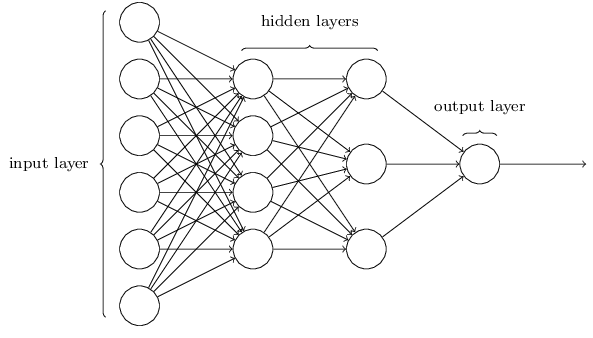
\includegraphics[scale=0.5]{network}

In general, we are trying to find a $\widehat{f}(x)$ to estimate $f(x)$ for any given $x$, where $x$, $\widehat{f}(x)$, and $f(x)$ may be vectors. To do this we minimize the cost:

$$ C(\widehat{f}, f) = \frac{1}{n} \sum_i C_x$$

where $C_x = L(\widehat{f}(x), f(x))$.

For example, the quadratic loss:

$$ C_x = \| \widehat{f}(x) - f(x) \|_2^2 $$

In a neural network, it is typical to call the outputs of each node its activations, where $a_k^l$ is the output of the $k^{th}$ node in the $l^{th}$ layer. Thus $a^L$ is the vector output of a network with $L$ layers.

Thus for a given training pair $(x,y)$ we seek to minimize

$$ C_x = \| a^L - y \|_2^2 $$

where $a^L$ is a function of $x$.

\subsection*{Perceptrons}

Activation function:

$$a(z) = I\{z > 0\}, \quad z = wx + b $$

Perceptrons can compute any function, so they are `universal for computation'.

But the activation function, being a step function, is too sensitive to small changes in the weights. This makes learning difficult...

\subsection*{Sigmoid neurons}

Activation function:

$$a(z) = \frac{1}{1 + exp(-z)}, \quad z = wx + b $$

Now, changes in the output are linear functions of the changes in the weights. This is good for learning.

\subsection*{Gradient descent}

To minimize some function $C$ we can start with some guess, $v$, and use gradient descent to update $v$ to $v' = v + \Delta v$ so that $C(v') < C(v)$.

To choose $\Delta v$, note that you want to change $v$ in the direction of the gradient: So if $\nabla C_v$ is the gradient of $C$ at $v$, then you want to set $\Delta v \propto -\nabla C_v$, i.e.:

$$v' = v - \eta \nabla C_v$$

where $\eta > 0$ is the `learning rate'.

If $\eta$ is too small, it will take a while to find the minimizer of $C$. On the other hand, if it's too large, you might overshoot the minimum.

In terms of our neural network, this means we update:

$$ w_k' = w_k - \eta \frac{\delta C}{\delta w_k}$$

$$ b_k' = b_k - \eta \frac{\delta C}{\delta b_k}$$

Recall that $C = \frac{1}{n} \sum_i C_x$. Thus we have

$$\frac{\delta C}{\delta b_k} = \frac{1}{n} \sum_i \frac{\delta C_x}{\delta b_k}$$

\subsubsection*{Stochastic gradient descent}

To compute $\nabla C$ we need to compute $\nabla C_x$, the gradient for each training point. So to speed up the process of making it through one update, we can just consider a subset of the total data. This is called stochastic gradient descent. Here's the outline:

\begin{enumerate}
\item Divide your data set $X$ into $m$ partitions, $X_1, ..., X_m$.
\item Using the data in $X_1$, calculate $\nabla C$, and update your weights and biases using the gradient descent step.
\item Now repeat on $X_2$, $X_3$, etc. Each of these steps you take is called a ``\textit{mini-batch}''.
\item Once you've used every partition to take a single gradient descent step, you've completed an ``\textit{epoch}''.
\end{enumerate}

\section*{Chapter 2}

\subsection*{Assumptions about the cost function}

To use backpropogration we must have two things:

\begin{enumerate}
\item a cost function that can be written as $C = \overline{C_x}$, where $C_x$ is the loss associated with each training input $x$.

\item The cost, $C_x$, of each training input must be a function only of the outputs of the network, $a^L$.
\end{enumerate}

Note that $a^L$ can be a vector if there are multiple outputs, with $a^L_j$ being the output of the $j^{th}$ in the last layer $L$.

Indeed, both of these assumptions are satisfied for the quadratic (MSE) loss:

$$C_x = \frac{1}{2}\| y - a^L \|^2  = \frac{1}{2n}\sum_j (y_j - a^L_j)^2$$

\subsection*{Backpropagation equations}

Because $C$ is just a sum over $C_x$, likewise $\nabla C$ is just a sum over $\nabla C_x$. In other words, we just need to know how some input $x$ affects $\nabla C_x$, and therefore determines $\frac{\delta C_x}{\delta w^l_{jk}}$ and $\frac{\delta C_x}{\delta b^l_k}$.

We'll first try to find the gradient of $C_x$ with respect to the weighted input to a node, $z^l_{k}$. Recall that $z^l_{k} = w^l_{k} a^{l-1} + b^l_k$. So once we have $\frac{\delta C_x}{\delta z^l_{k}}$, clearly the following is true:

\begin{equation}
\frac{\delta C_x}{\delta b^l_{k}} = \frac{\delta C_x}{\delta z^l_{jk}}
\end{equation}

\begin{equation}
\frac{\delta C_x}{\delta w^l_{jk}} = \frac{\delta C_x}{\delta z^l_{jk}}a^{l-1}_{j}
\end{equation}

So now we just need $\frac{\delta C_x}{\delta z^l_{k}}$. The gradient of the output of the network is the easiest place to start. We can then work backwards to get the gradient for earlier layers. Hence, ``backpropagation''.

Recall that our cost function, $C_x$, is solely a function of the output of our network, $a^L$. So letting our activation function be $\sigma(.)$, then the output of our network is $a^L = \sigma(z^L)$. Thus:

\begin{equation}
\frac{\delta C_x}{\delta z^L_k} = \frac{\delta C_x}{\delta a^L_k} \sigma'(z^L_k)
\end{equation}

We now just to need to find $\frac{\delta C_x}{\delta z^{l}_k}$ given $\frac{\delta C_x}{\delta z^{l+1}_k}$, and we're done.

\begin{equation}
\frac{\delta C_x}{\delta z^l_k} = w^{l+1}_{.,k}\frac{\delta C_x}{\delta z^{l+1}} \sigma'(z^l_k)
\end{equation}

where $w^{l+1}_{.,k}$ is the vector of weights from the $(l+1)^{th}$ layer on the outputs of $a^l_k$, and $\frac{\delta C_x}{\delta z^{l+1}}$ is the vector form of the previous equation.

\subsection*{Gradient descent with backpropagation algorithm}

\begin{enumerate}
\item Given a set of $m$ training examples (e.g., a mini-batch). For each training example $x$, calculate its contribution to the gradient:
\subitem Feedforward: for each $l = 2, 3, ... L$ compute $z^{x,l}= w^l a^{x,l-1} + b^l$, and $a^{x,l} = \sigma(z^{x,l})$.
\subitem Calculate the output error vector: $\delta^{x,L} = \nabla_a \odot C_x \sigma'(z^{x,l})$
\subitem Backpropagate the error: for each $l = L-1, L-2, ..., 2$ compute $\delta^{x,l} = ((w^{l+1})^T\delta^{x,l+1})\odot \sigma'(z^{x,l})$
\item Gradient descent: for each $l = L, L-1, ..., 2$ update the weights $w^l \to w^l - \frac{\eta}{m} \sum_x \delta^{x,l}(a^{x,l-1})^T$, and $b^l \to b^l - \frac{\eta}{m} \sum_x \delta^{x,l}$.
\end{enumerate}

\section*{Chapter 3}

\subsection*{Cost functions and output activations}

\subsubsection*{Sigmoid activation and cross-entropy loss}

Recall our MSE loss/cost function (also called quadratic loss):

$$ C_x = \| y - a \|^2 $$

Recall that for this loss, the gradient of our weights and biases is proportional to $a'(z)$, the derivative of your activation function. If our activation function is a sigmoid, as below, notice that whenever our weighted input $z$ gets too large or too small, $a'(z)$ will be near $0$.

This is problematic because our intuition is that the further our estimated output is from the true output, the quicker we should learn. But if you consider the case where our output is $y=1$ and our input is $x=0$, then $z = wx+b$ will be small and so our $a'(z)$ will also be small. But our gradient is proportional to $a'(z)$, and so we will not learn that quickly!

Enter the cross-entropy loss function:

$$ C_x = y\ln(a) + (1-y)\ln(1-a) $$

Then with a sigmoid activation function, our gradients are now proportional to $y - a$, i.e., the error in our outputs. Perfect!


\subsubsection*{Output activation functions}

Sometimes you can have a different output activation function than your other layers' activation function. This will in turn change the way the gradient depends on errors.

Here are various combinations that lead to a gradient proportional to the error, $y - a$:

\begin{enumerate}

\item Cross-entropy loss + sigmoid output activation
\item Quadratic loss + linear output activation (i.e., $a(z) = z$)
\item log-likelihood loss + softmax output activation (i.e., $a(z)$ is like a sigmoid but then it's normalized across outputs so that the sum of all outputs is $1$)

\end{enumerate}


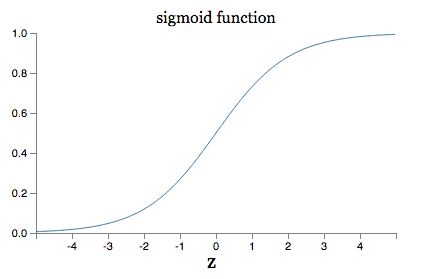
\includegraphics[scale=0.5]{sigmoid}


\subsection*{Regularization}

``The obvious way to detect overfitting is to [keep] track of accuracy on the test data as our network trains. If we see that the accuracy on the test data is no longer improving, then we should stop training.''

\subsubsection*{$L_1$ and $L_2$ regularization}

If your cost function is $C_0$, then the $L_p$ regularized cost function is

$$ C = C_0 + \frac{\lambda}{2n}\| w \|_p $$

where typically $p = 1$ or $2$.

``When $\lambda$ is small we prefer to minimize the original cost function, but when $\lambda$ is large we prefer small weights.''

For $L_2$ regularization, this is sometimes called `weight decay' because the regularized cost function results in a weight update that looks like

$$ w \to (1 - \frac{\eta\lambda}{n})w- \eta \nabla_w $$

In other words, $w$ will shrink over time unless the $\eta \nabla_w$ term compensates.

Note that for $L_1$, the update is

$$ w \to w - \frac{\eta\lambda}{n}sign(w)- \eta \nabla_w $$

``In L1 regularization, the weights shrink by a constant amount toward $0$. In L2 regularization, the weights shrink by an amount which is proportional to $w$. And so when a particular weight has a large magnitude, $|w|$, L1 regularization shrinks the weight much less than L2 regularization does. By contrast, when $|w|$ is small, L1 regularization shrinks the weight much more than L2 regularization. The net result is that L1 regularization tends to concentrate the weight of the network in a relatively small number of high-importance connections, while the other weights are driven toward zero.''

\subsubsection*{Dropout}

It's amazing that dropout works at all: Instead of modifying the cost function, you instead knock out half of your network (i.e., you simply eliminate half of all your nodes, temporarily). You then train with this smaller network for an entire mini-batch, and then you restore your network, randomly delete more nodes, and then repeat.

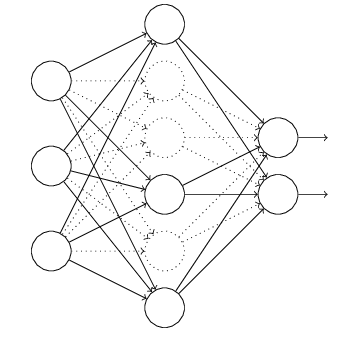
\includegraphics[scale=0.8]{dropout}

Because you're now training with fewer nodes, your weights will be larger, so in the end you just halve the weights.


How does it work? Here's one intuition, from a Hinton paper: ``This technique reduces complex co-adaptations of neurons, since a neuron cannot rely on the presence of particular other neurons. It is, therefore, forced to learn more robust features that are useful in conjunction with many different random subsets of the other neurons.''

\subsubsection*{Adding artificial input data}

There are often many trivial ways of creating more input data. For example, if you're training on images, simply rotate all of them! So if you've got images of a hand-written $5$, you can rotate, stretch, and translate the $5$ and they will all be different inputs as far as your model can tell.

\subsubsection*{Comments on over-fitting}

\begin{enumerate}
\item ``The Nobel prizewinning physicist Enrico Fermi was once asked his opinion of a mathematical model some colleagues had proposed as the solution to an important unsolved physics problem. The model gave excellent agreement with experiment, but Fermi was skeptical. He asked how many free parameters could be set in the model. `Four' was the answer. Fermi replied: `I remember my friend Johnny von Neumann used to say, with four parameters I can fit an elephant, and with five I can make him wiggle his trunk.'.''


\item Fitting $99$ points with a line versus a $99^{th}$ order polynomial: ``Which of these is the better model? Which is more likely to be true? And which model is more likely to generalize well to other examples of the same underlying real-world phenomenon?

...In fact, we can't determine with certainty the answer to any of the above questions, without much more information about the underlying real-world phenomenon. But let's consider two possibilities: (1) the 99th order polynomial is, in fact, the model which truly describes the real-world phenomenon, and the model will therefore generalize perfectly; (2) the correct model is y=2x, but there's a little additional noise due to, say, measurement error, and that's why the model isn't an exact fit.

It's not a priori possible to say which of these two possibilities is correct. (Or, indeed, if some third possibility holds). Logically, either could be true...One point of view is to say that in science we should go with the simpler explanation, unless compelled not to.''

\item Why do neural networks not overfit? ``A network with 100 hidden neurons has nearly 80,000 parameters. We have only 50,000 images in our training data. It's like trying to fit an 80,000th degree polynomial to 50,000 data points. By all rights, our network should overfit terribly. And yet, as we saw earlier, such a network actually does a pretty good job generalizing. Why is that the case? It's not well understood.''

\item The human brain must regularize, too: ``We humans generalize phenomenally well. Shown just a few images of an elephant a child will quickly learn to recognize other elephants. Of course, they may occasionally make mistakes, perhaps confusing a rhinoceros for an elephant, but in general this process works remarkably accurately. So we have a system - the human brain - with a huge number of free parameters. And after being shown just one or a few training images that system learns to generalize to other images. Our brains are, in some sense, regularizing amazingly well! How do we do it? At this point we don't know.''

\end{enumerate}

\subsection*{Initializing weights and other optimization techniques}

\begin{enumerate}
\item Initialize weights and biases as $\sim N(0, \sigma^2)$, where $\sigma^2$ is narrow enough that most of your activations aren't saturated. Typically, set $\sigma^2 = 1/\sqrt{n_{in}}$, where $n_{in}$ is the number of inputs to a given node.
\item Some people have the learning rate shrink as your number of epochs increase.
\item Momentum-based stochastic gradient descent: Usually better.
\item tanh() instead of logistic(): Might be better, might be not.
\item ReLu(z) = max(0, z): Good for image recognition
\end{enumerate}

\subsection*{Choosing hyperparameters}

Basically, he suggests that the main problem of neural networks is at the very beginning: You just want to get \textit{any} learning. To attack this problem:

\begin{enumerate}
\item Simplify your inputs (e.g., if you're doing classification, remove all but two classes from your training data)
\item Simplify your network (e.g., remove your hidden layer)
\item Find the right learning rate.
\end{enumerate}

Then you can slowly add in complexity and mess around with any other hyperparameters, like regularization, for example.

\section*{Chapter 4}

A visual proof that neural nets can compute any function, i.e., the universality of a neural network.

The basic idea is that you (1) figure out how your weights/biases work, then you mess around with that until you can (2) use them to make a step function, and then you make a series of step functions which allows you to (3) capture any function $f(x)$ with its discretized approximation.

\begin{enumerate}

\item
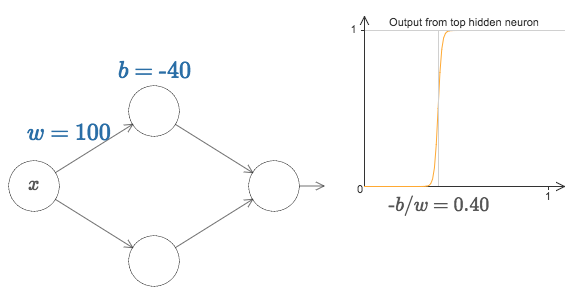
\includegraphics[scale=0.5]{universality-1a}

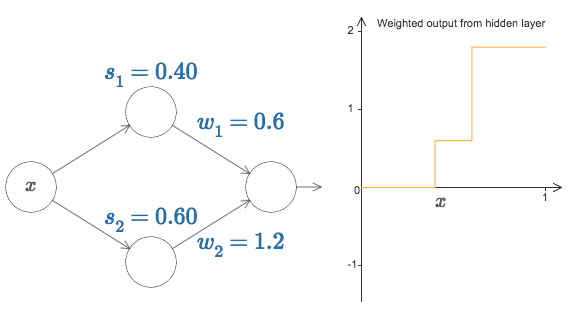
\includegraphics[scale=0.5]{universality-1b}
\item
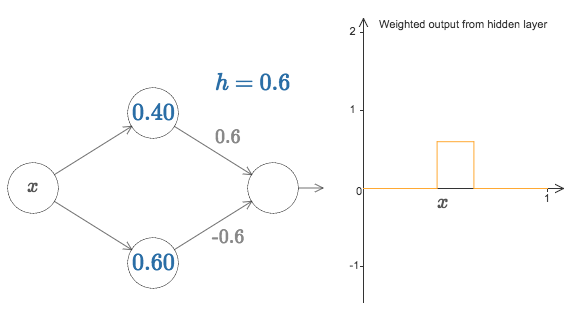
\includegraphics[scale=0.5]{universality-2}
\item
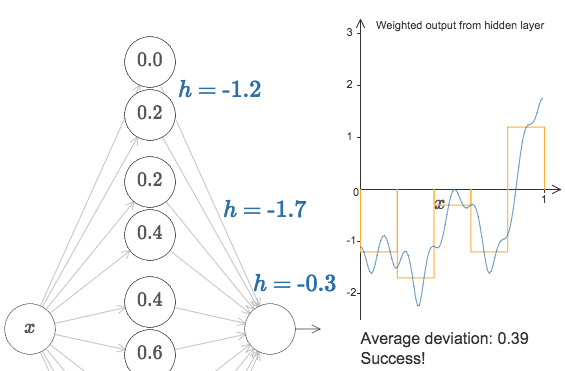
\includegraphics[scale=0.5]{universality-3}

\end{enumerate}


\section*{Chapter 5}

The unstable gradient problem: The more hidden layers, the more learning in the last layer relative to the first layer.

You can measure the amount of learning by looking at $\| \delta^l \|$ for each layer $l$, where $\delta_i^l$ is $\delta C/\delta z_i^l$, i.e., the gradient of the cost with respect to the weighted input to the $i^{th}$ node in the $l^{th}$ layer.

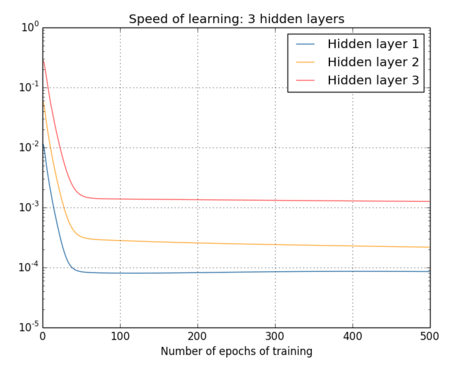
\includegraphics[scale=0.8]{vanishing-gradient}

The reason for this is best seen in the cast where each layer has exactly one node. Consider $\delta_i^l = \delta C/\delta z_i^l = \delta C/\delta b_i^l$ below, for the first layer $l=1$:

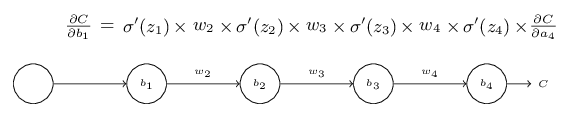
\includegraphics[scale=0.8]{product-of-gradients}

Note the successive products of $\sigma'(z_i)w_i$: If this value is on average below $1$, the gradient will tend to vanish as you add more layers; if this value is above $1$, it will tend to explode.

\section*{Chapter 6}

\subsection*{Convolutional neural networks}

Often for convolutional neural networks people use a ReLu activation function, just because it tends to do better than a sigmoid.

\subsubsection*{Local receptive fields}

Before, we visualized each layer as a vector. Here, it's best to visualize it as a matrix. Now, each neuron in the hidden layer will be connected to a small region of the input neurons--for example, a $5 \times 5$ region. That region is called the neuron's \textit{receptive field}.

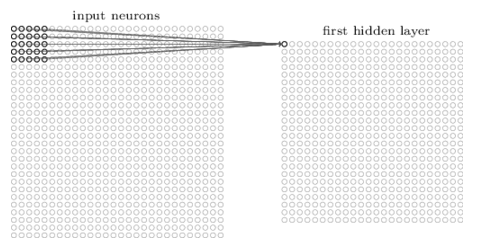
\includegraphics[scale=0.8]{receptive-field.png}

The next neuron in the hidden layer will have a receptive field that slightly overlaps with the other nearby neurons' receptive fields. The \textit{stride length} specifies by how much neighboring receptive fields overlap.


\subsubsection*{Convolutional layers = shared weights}

Each neuron in a hidden layer has the same size receptive field. Critically, in a convolutional neural network, each of these neurons uses the \textit{same} weights and bias.

In other words, the below equation is the output for the $(x,y)^{th}$ hidden neuron, where $w$ is a $5 \times 5$ array of shared weights:

$$ \sigma\left( b + \sum_{i=1}^5 \sum_{j=1}^5 w_{i,j}a_{x+i,y+j} \right) $$

This means that ``all the neurons in a hidden layer detect exactly the same feature, just at different locations in the input image.'' For this reason, the shared weights are often called a `feature map', `kernel' or `filter'. The process of applying the same weights to all positions in the input image is called a ``convolution''.

Here's an example of some feature maps a network might learn:

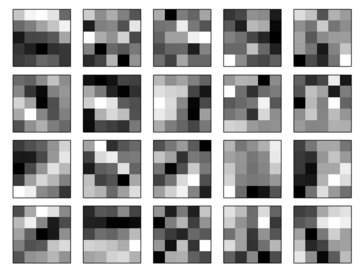
\includegraphics[scale=0.8]{feature-maps.png}

A big advantage of convolutional layers is thus that there are far fewer parameter values to learn.

\subsubsection*{Pooling}

Pooling layers are often used immediately after convolutional layers. Each unit in the pooling layer summarizes a region of, say, $2 \times 2$ neurons in the previous layer.

\begin{enumerate}
\item \textit{max-pooling} - outputs the maximum activation in its receptive field
\item \textit{L2 pooling} - outputs the square root of the sum of the activations in its receptive field
\end{enumerate}

``We can think of max-pooling as a way for the network to ask whether a given feature is found anywhere in a region of the image. It then throws away the exact positional information. The intuition is that once a feature has been found, its exact location isn't as important as its rough location relative to other features. A big benefit is that there are many fewer pooled features, and so this helps reduce the number of parameters needed in later layers.''

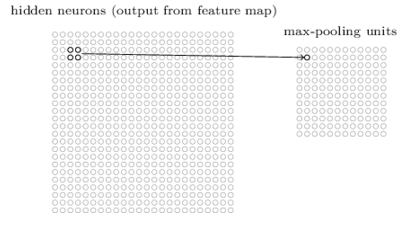
\includegraphics[scale=0.8]{pooling.png}

\subsubsection*{Putting it all together}

\begin{figure}[!ht]
    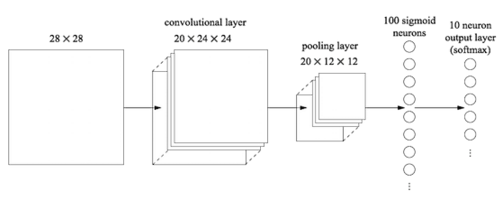
\includegraphics[scale=0.8]{conv-simple.png}
    \centering

    A simple convolutional network with two fully connected layers.
\end{figure}

\begin{figure}[!ht]
    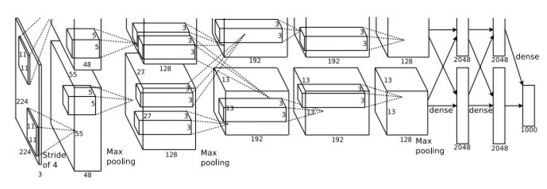
\includegraphics[scale=0.8]{conv.png}

    \centering
    An example of a full convolutional network model (implemented on 2 GPUs).
\end{figure}

\subsection*{Adversarial images}

``A 2013 paper showed that deep networks may suffer from what are effectively blind spots. Consider the lines of images below. On the left is an ImageNet image classified correctly by their network. On the right is a slightly perturbed image (the perturbation is in the middle) which is classified incorrectly by the network. The authors found that there are such `adversarial' images for every sample image, not just a few special ones.''

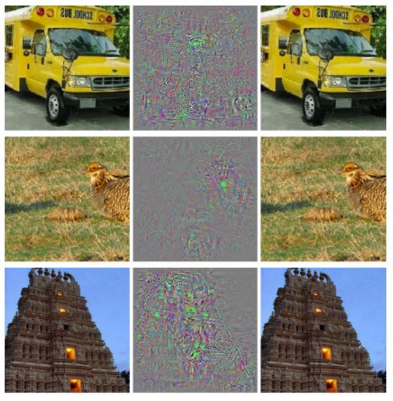
\includegraphics[scale=0.8]{adversarial.png}

``While such neural networks compute functions which are, in principle, continuous, results like this suggest that in practice they're likely to compute functions which are very nearly discontinuous.''

\subsection*{Other neural network types}

\begin{enumerate}
\item \textit{recurrent neural networks (RNNs)} - behavior of hidden neurons determined by activations at previous layers \textit{and} its own activation at an earlier time
\item \textit{Long short-term memory units (LSTMs)} - solve the RNN's unstable gradient problem
\item \textit{Deep belief nets (DBNs), generative models, and Boltzmann machines} - allow you to `run the network backward' and generate other input values creating the same input activations; can do both unsupervised and semi-supervised learning
\end{enumerate}

\end{document}
